\documentclass[tikz,border=10pt]{standalone}
\usepackage{tikz}
\usetikzlibrary{arrows.meta,positioning,fit,backgrounds,calc,shadows,shapes.geometric}

\definecolor{civNavy}{RGB}{15, 34, 64}
\definecolor{civBlue}{RGB}{28, 80, 160}
\definecolor{civTeal}{RGB}{14, 130, 120}
\definecolor{civLightBlue}{RGB}{238, 245, 255}
\definecolor{civGold}{RGB}{217, 119, 6}
\definecolor{civGreen}{RGB}{22, 130, 80}
\definecolor{civDark}{RGB}{20, 28, 42}

\begin{document}
% Gantt Chart for CiviQ Project Implementation
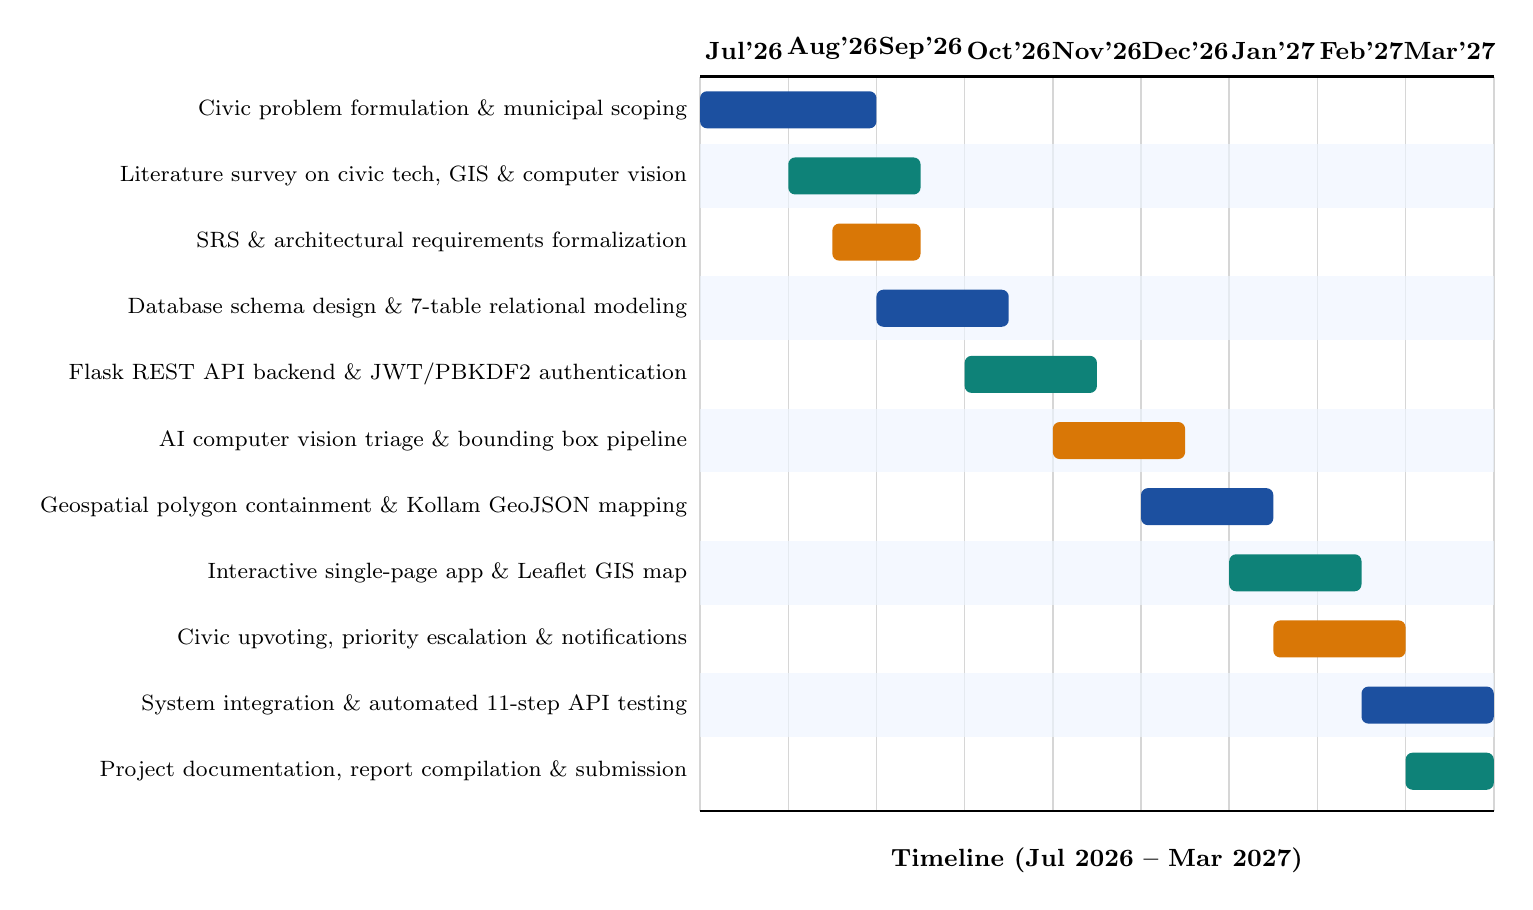
\begin{tikzpicture}[
  x=1.12cm, y=0.84cm,
  lab/.style={anchor=east, font=\fontsize{8.5}{10.5}\selectfont, inner sep=4.5pt, text=black}
]
\def\nm{9}
\def\topY{11.5}

% Vertical month gridlines
\foreach \i in {0,1,...,\nm} {
  \draw[gray!32, line width=0.55pt] (\i, 0.4) -- (\i, \topY);
}

% Month headers on top
\foreach \i/\m in {0.5/Jul'26, 1.5/Aug'26, 2.5/Sep'26, 3.5/Oct'26, 4.5/Nov'26, 5.5/Dec'26, 6.5/Jan'27, 7.5/Feb'27, 8.5/Mar'27} {
  \node[anchor=south, font=\fontsize{9.0}{11.0}\selectfont\bfseries, text=black] at (\i, \topY+0.12) {\m};
}
\draw[black, line width=1.0pt] (0, \topY) -- (\nm, \topY);
\draw[black, line width=0.8pt] (0, 0.4) -- (\nm, 0.4);

% Alternating row background shading
\foreach \k in {0,...,10} {
  \pgfmathsetmacro{\yc}{11.0-\k}
  \ifodd\k
    \fill[civLightBlue, opacity=0.65] (0, \yc-0.48) rectangle (\nm, \yc+0.48);
  \fi
}

% Task milestone labels on left
\node[lab] at (0, 11.0) {Civic problem formulation \& municipal scoping};
\node[lab] at (0, 10.0) {Literature survey on civic tech, GIS \& computer vision};
\node[lab] at (0, 9.0)  {SRS \& architectural requirements formalization};
\node[lab] at (0, 8.0)  {Database schema design \& 7-table relational modeling};
\node[lab] at (0, 7.0)  {Flask REST API backend \& JWT/PBKDF2 authentication};
\node[lab] at (0, 6.0)  {AI computer vision triage \& bounding box pipeline};
\node[lab] at (0, 5.0)  {Geospatial polygon containment \& Kollam GeoJSON mapping};
\node[lab] at (0, 4.0)  {Interactive single-page app \& Leaflet GIS map};
\node[lab] at (0, 3.0)  {Civic upvoting, priority escalation \& notifications};
\node[lab] at (0, 2.0)  {System integration \& automated 11-step API testing};
\node[lab] at (0, 1.0)  {Project documentation, report compilation \& submission};

% Milestone Gantt Bars
\fill[civBlue, rounded corners=2.5pt]     (0.0, 11.0-0.28) rectangle (2.0, 11.0+0.28);
\fill[civTeal, rounded corners=2.5pt]     (1.0, 10.0-0.28) rectangle (2.5, 10.0+0.28);
\fill[civGold, rounded corners=2.5pt]     (1.5, 9.0-0.28)  rectangle (2.5, 9.0+0.28);
\fill[civBlue, rounded corners=2.5pt]     (2.0, 8.0-0.28)  rectangle (3.5, 8.0+0.28);
\fill[civTeal, rounded corners=2.5pt]     (3.0, 7.0-0.28)  rectangle (4.5, 7.0+0.28);
\fill[civGold, rounded corners=2.5pt]     (4.0, 6.0-0.28)  rectangle (5.5, 6.0+0.28);
\fill[civBlue, rounded corners=2.5pt]     (5.0, 5.0-0.28)  rectangle (6.5, 5.0+0.28);
\fill[civTeal, rounded corners=2.5pt]     (6.0, 4.0-0.28)  rectangle (7.5, 4.0+0.28);
\fill[civGold, rounded corners=2.5pt]     (6.5, 3.0-0.28)  rectangle (8.0, 3.0+0.28);
\fill[civBlue, rounded corners=2.5pt]     (7.5, 2.0-0.28)  rectangle (9.0, 2.0+0.28);
\fill[civTeal, rounded corners=2.5pt]     (8.0, 1.0-0.28)  rectangle (9.0, 1.0+0.28);

% Bottom title
\node[font=\fontsize{9.2}{11.2}\selectfont\bfseries, text=black] at (4.5, -0.35) {Timeline (Jul 2026 -- Mar 2027)};
\end{tikzpicture}
\end{document}
